\chapter{Results} 

\label{Chapter7} 

\lhead{Chapter 7. \emph{Results}}

\section{Performance}
Performance has been the main concern in the development of the system. As already seen in previous chapters, many efforts have been made in order to achieve a good responsiveness to user input in the real time application. We made the clear choice of preferring low times in the offline computation of descriptors (reported in Table~\ref{table:benchmarkoffline}) for this has helped us in achieving good response times in the real time application. The latter ones, in general, greatly vary with the use of the application. For instance, the user interaction with sliders has the effect of emptying the playlist queue (which will result in temporary shorter computational times, due to the use of the least precise but fastest music similarity computation algorithm in order to get some new element into the playlist as soon as possible), while choosing to use longer segments or not interacting with the sliders may increase the computational time (for the system realizes that it has more time available for computing music similarity and then uses the most accurate algorithm\footnote{We recall that the only difference between the two algorithms lies in the choice of the similarity function, as shown at the point 8 of Section~\ref{subsec:rtalgorithm}}). \\
For us, this instability of performance is not intended as a flaw: it could rather be seen as good flexibility of the system to many different computational situations.\\
We decided to collect data about computational times of the real time application for the choice of 1000 consecutive excerpts, with occasional interaction of the user. This is a reasonable analysis case, for it may be very similar to the real use of the system and also provides a good perspective on the computational times while using the most demanding algorithm of the system for computing music similarity. The results are shown for each main point of the procedure explained in Section~\ref{subsec:rtalgorithm}.



\begin{figure}[h]
\begin{center}
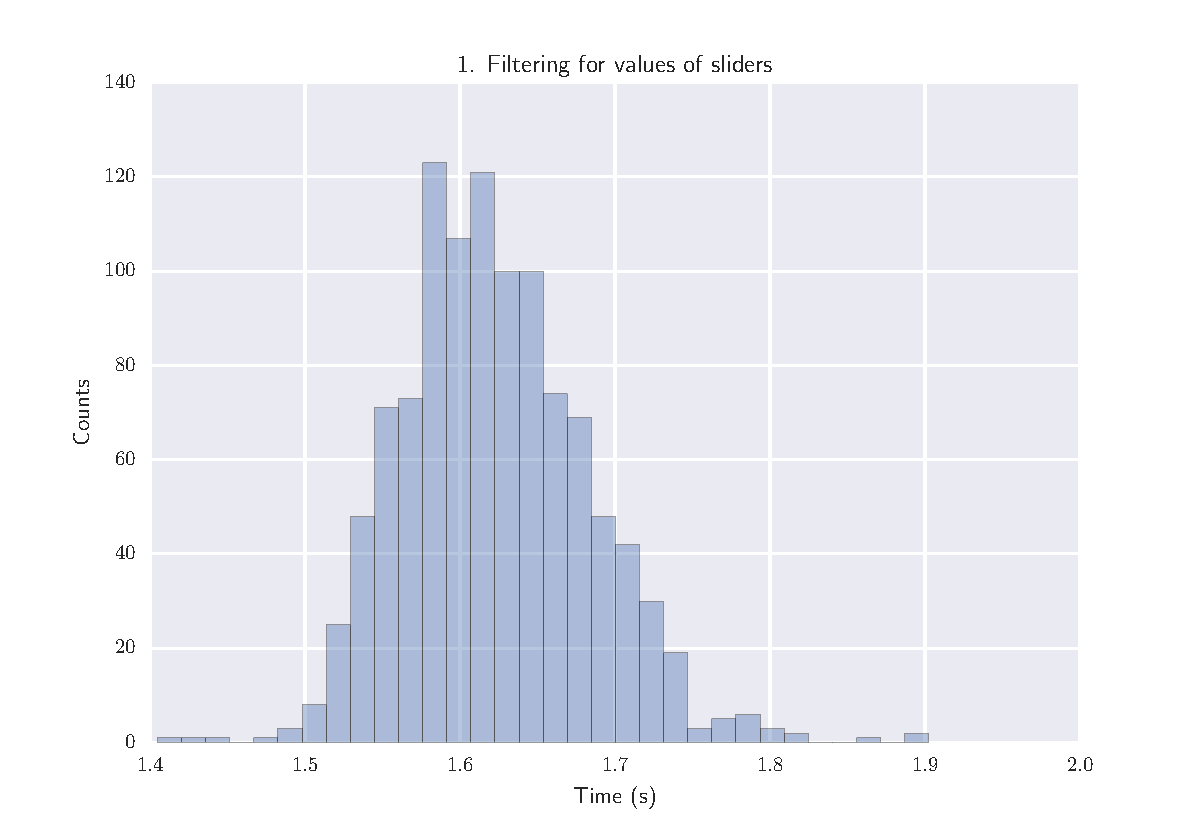
\includegraphics[scale=0.7]{Figures/bench_sliders.pdf}
    \rule{10em}{0.5pt}
  \caption[Time for filtering music in regards to sliders' positions]{Time for performing the first step of the procedure: filtering of excerpts based on the current positions of sliders.}
  \label{fig:step1}
\end{center}
\end{figure}

\begin{figure}[h]
\begin{center}
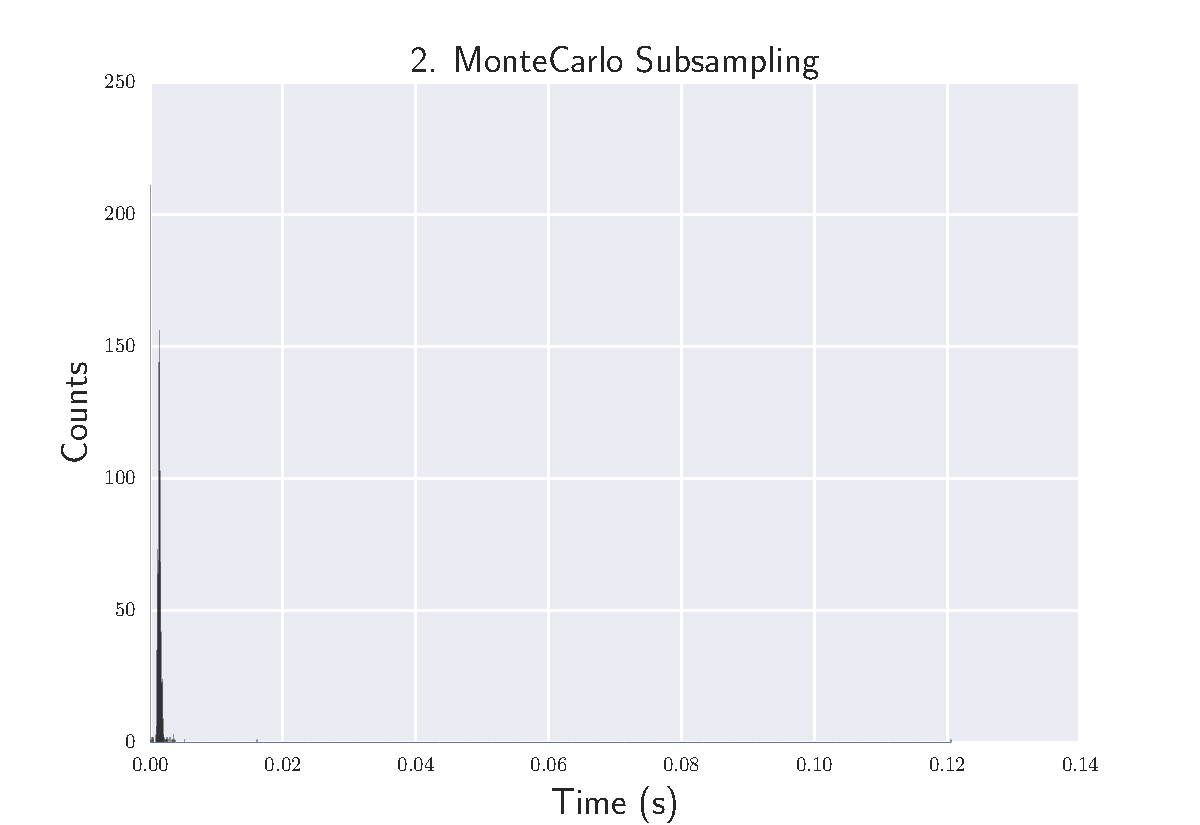
\includegraphics[scale=0.7]{Figures/bench_subsampling.pdf}
    \rule{10em}{0.5pt}
  \caption[Time for performing Monte Carlo subsampling]{Time for performing Monte Carlo subsampling.}
  \label{fig:step2}
\end{center}
\end{figure}

\begin{figure}[h]
\begin{center}
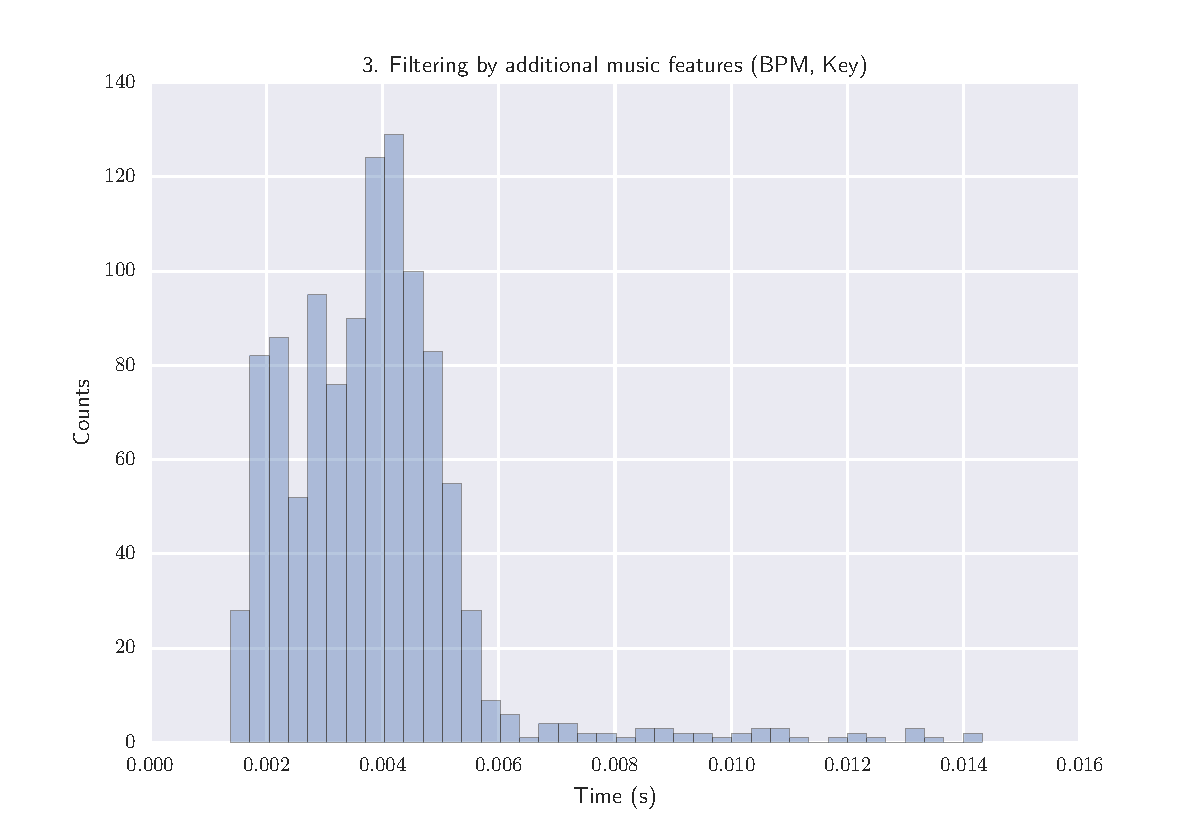
\includegraphics[scale=0.7]{Figures/bench_bpm_filters.pdf}
    \rule{10em}{0.5pt}
  \caption[Time for filtering music according to musicality with current excerpt]{Time for filtering music according to musicality with current excerpt (in regards of BPM and key).}
  \label{fig:step3}
\end{center}
\end{figure}

\begin{figure}[h]
\begin{center}
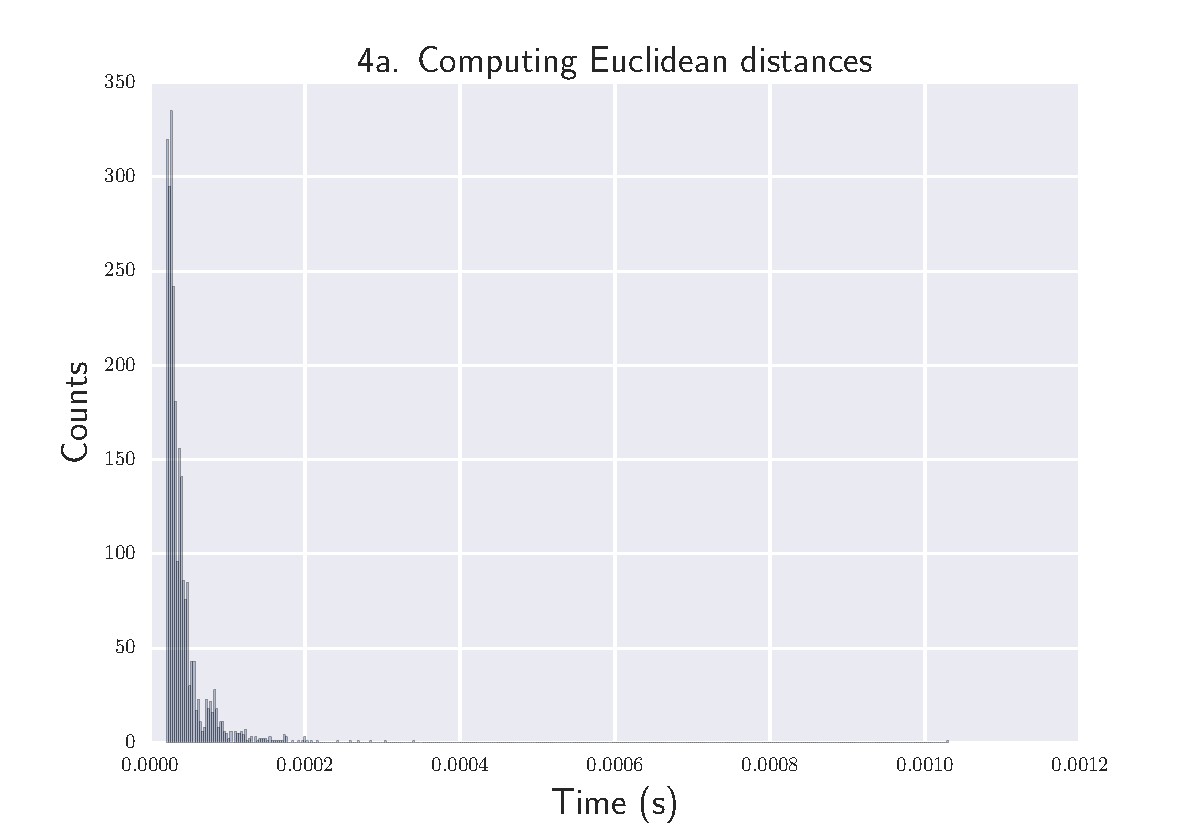
\includegraphics[scale=0.7]{Figures/bench_euclidean.pdf}
    \rule{10em}{0.5pt}
  \caption[Time for computing euclidean distance]{Time for computing euclidean distance between two 20D points.}
  \label{fig:step4}
\end{center}
\end{figure}

\begin{figure}[h]
\begin{center}
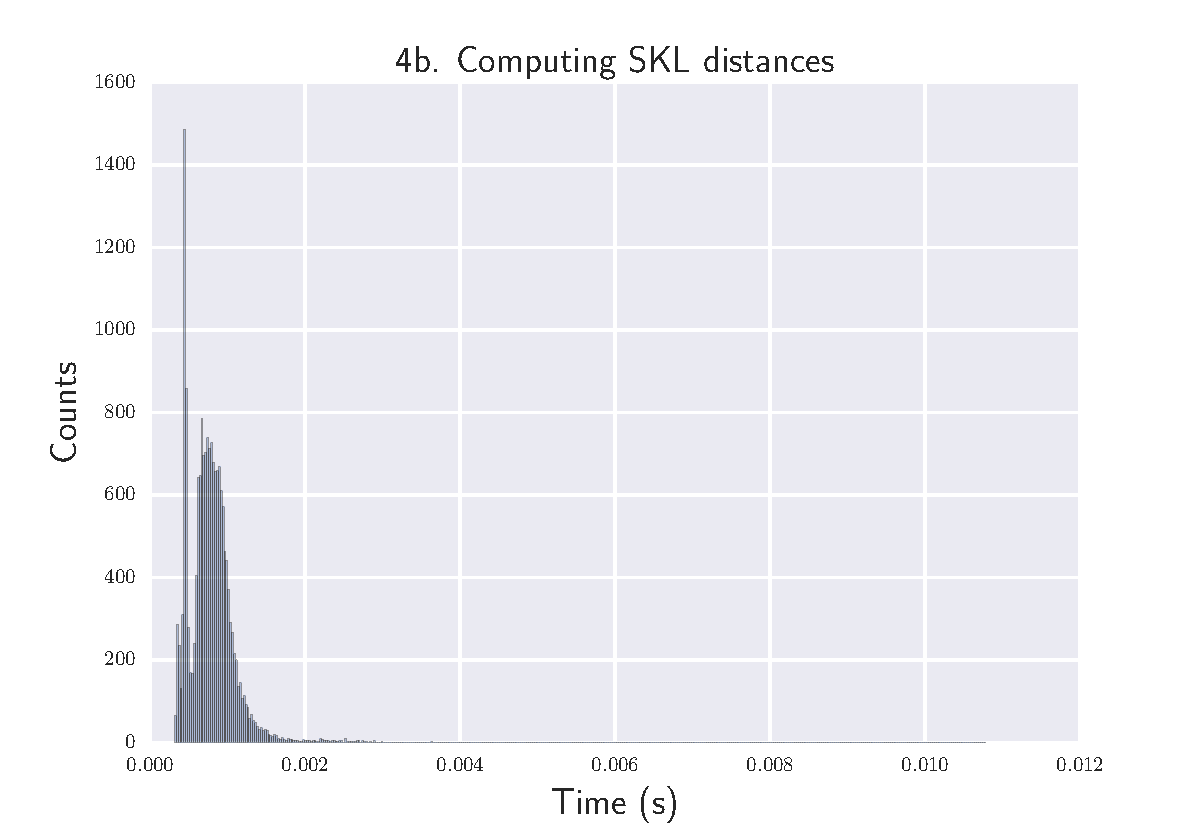
\includegraphics[scale=0.7]{Figures/bench_skl.pdf}
    \rule{10em}{0.5pt}
  \caption[Time for computing symmetric Kullback-Leibler distance]{Time for computing symmetric Kullback-Leibler distance between two excerpts.}
  \label{fig:step5}
\end{center}
\end{figure}

\begin{figure}[h]
\begin{center}
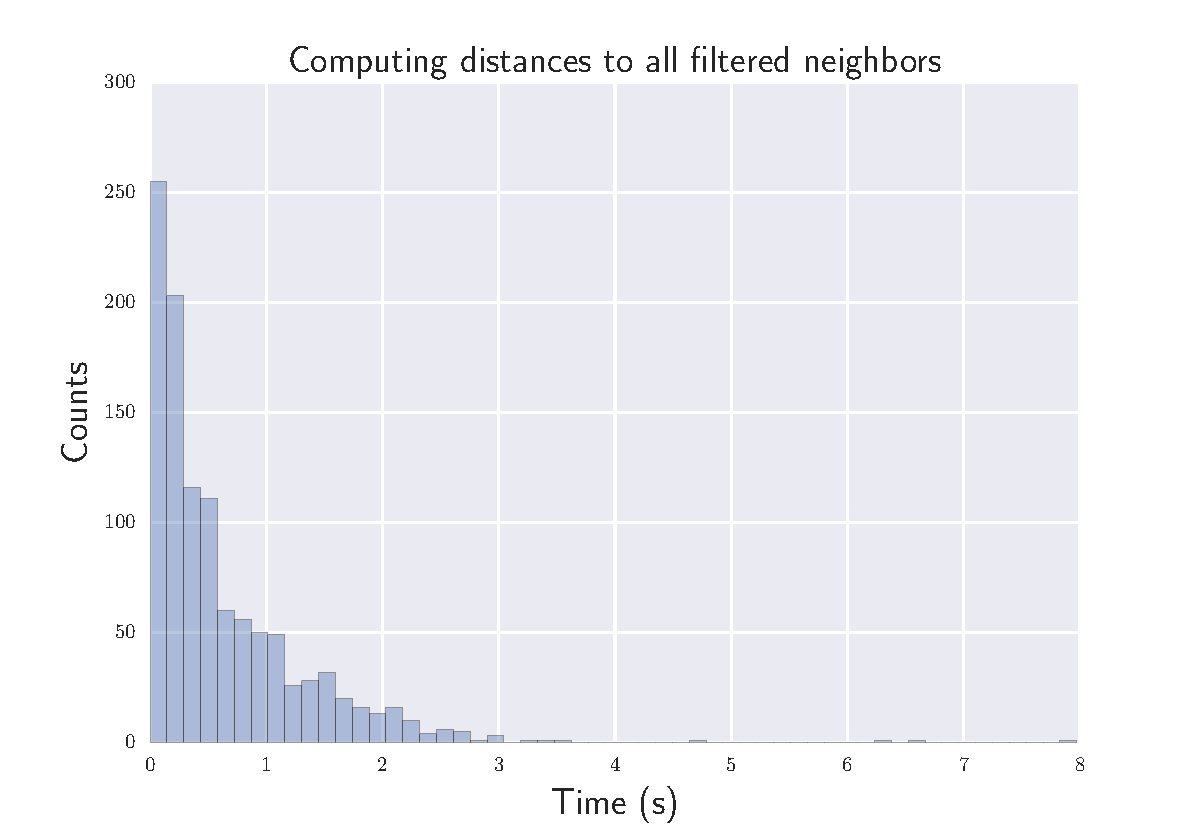
\includegraphics[scale=0.7]{Figures/bench_get_suitsegm.pdf}
    \rule{10em}{0.5pt}
  \caption[Time for computing distances from all filtered segments]{Time for computing distances from all filtered segments.}
  \label{fig:step6}
\end{center}
\end{figure}

\begin{figure}[h]
\begin{center}
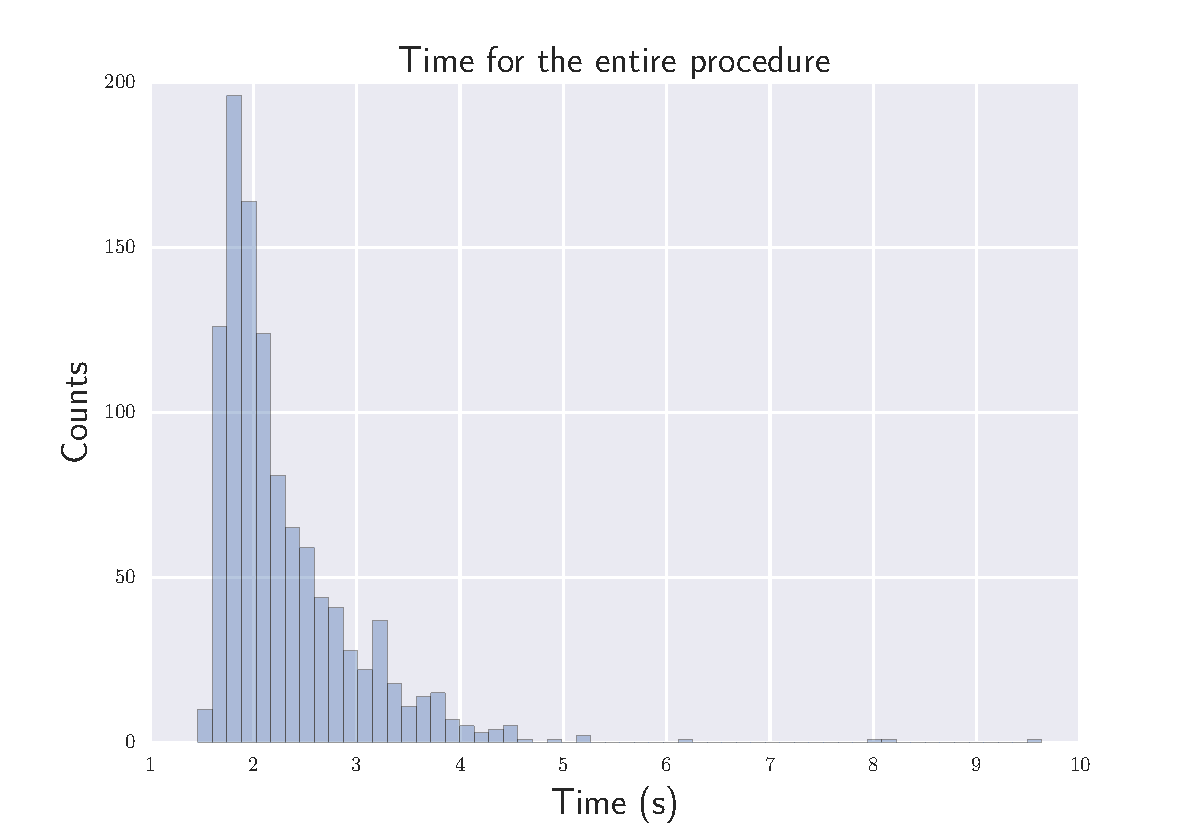
\includegraphics[scale=0.7]{Figures/bench_procedure.pdf}
    \rule{10em}{0.5pt}
  \caption[Global time for selecting next segment]{Global time for selecting next segment.}
  \label{fig:step7}
\end{center}
\end{figure}

\begin{figure}[h]
\begin{center}
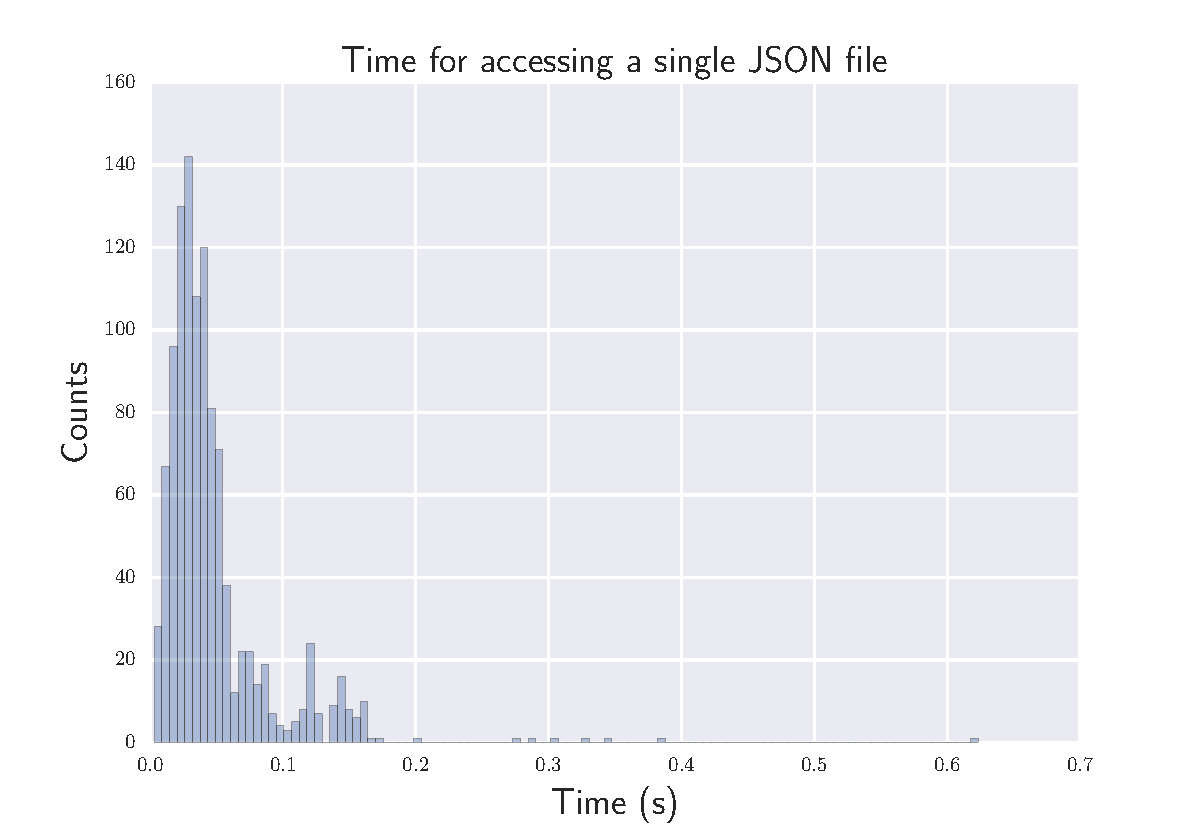
\includegraphics[scale=0.7]{Figures/bench_json_single.pdf}
    \rule{10em}{0.5pt}
  \caption[Time for accessing and parsing a JSON file]{Time for accessing and parsing a JSON file.}
  \label{fig:step8}
\end{center}
\end{figure}






\section{Evaluation}
\section{Use at exhibition} 
\section{Results obtained by the study}